% appendixd.tex
% This work is licensed under the Creative Commons Attribution-Noncommercial-Share Alike 3.0 New Zealand License.
% To view a copy of this license, visit http://creativecommons.org/licenses/by-nc-sa/3.0/nz
% or send a letter to Creative Commons, 171 Second Street, Suite 300, San Francisco, California, 94105, USA.


\chapter{Respuestas a ``Cosas que puedes probar''}\label{app:answers}

Aquí puedes encontrar las respuestas a las preguntas de la sección ``Cosas que puedes probar'' de cada capítulo.

\subsection*{Capítulo \ref{ch:8multipliedby3.57}}

1. La respuesta del \textbf{Ejercicio 1} podría ser como sigue:

\begin{listing}
\begin{verbatim}
>>> juguetes = [ 'coche', 'Nintendo Wii', 'ordenador', 'bicicleta' ]
>>> comidas = [ 'pasteles', 'chocolate', 'helado' ]
>>> favoritos = juguetes + comidas
>>> print(favoritos)
[ 'coche', 'Nintendo Wii', 'ordenador', 'bicicleta', 'pasteles', 'chocolate', 'helado' ]
\end{verbatim}
\end{listing}

\noindent
2.  La respuesta al \textbf{Ejercicio 2} consiste en sumar el resultado de multiplicar 3 por 25 y el resultado de multiplicar 10 por 32.   Las siguientes fórmulas muestran el resultado:

\begin{listing}
\begin{verbatim}
>>> print(3 * 25 + 10 * 32)
395
\end{verbatim}
\end{listing}

\noindent
Sin embargo, ya que miramos el uso de los paréntesis en el Capítulo 2, podrías utilizar paréntesis, aunque en esta fórmula no fuesen necesarios:

\begin{listing}
\begin{verbatim}
>>> print((3 * 25) + (10 * 32))
395
\end{verbatim}
\end{listing}

\noindent
La respuesta es la misma ya que en Python la multiplicación se hace siempre antes que la suma. Según hemos puesto los paréntesis, le estamos diciendo a Python que haga primero las multiplicaciones, que es lo mismo que pasa en el caso anterior sin los paréntesis.  Sin embargo la segunda fórmula queda más clara que la primera---porque aclara inmediatamente al que la lee qué operaciones se hacen antes.   Un programador con poco conocimiento (que no conozca el orden en que ejecuta Python las operaciones) podría pensar que en la primera ecuación lo que pasa es que se multiplica 3 por 25, luego se suma 10, y luego se multiplica el resultado por 32 (que daría como resultado 2720---y que es completamente equivocado).   Con los paréntesis queda un poquito más claro lo que se calcula antes.

\noindent
3.  La respuesta al \textbf{Ejercicio 3} será parecida a lo siguiente:

\begin{listing}
\begin{verbatim}
>>> nombre = 'Mary'
>>> apellidos = 'Wilson'
>>> print('Mi nombre es %s %s' % (nombre, apellidos))
Mi nombre es Mary Wilson
\end{verbatim}
\end{listing}

\subsection*{Capítulo \ref{ch:turtles}}

\noindent
1. Un rectángulo es como un cuadrado, excepto en que dos de sus lados son más largos que los otros dos.   Para dibujarlo con la tortuga habrá que decirle a la tortuga las siguientes operaciones:

\begin{itemize}
 \item muévete un número de píxeles.
 \item gira a la izquierda.
 \item muévete un número menor de píxeles.
 \item gira a la izquierda.
 \item muévete el mismo número de píxeles que en el primer movimiento.
 \item gira a la izquierda.
 \item muévete el número de píxeles del segundo movimiento.
\end{itemize}

\noindent
Por ejemplo, el siguiente código dibujará el rectángulo de la figura~\ref{fig46}.

\begin{listing}
\begin{verbatim}
>>> import turtle
>>> t = turtle.Pen()
>>> t.forward(150)
>>> t.left(90)
>>> t.forward(50)
>>> t.left(90)
>>> t.forward(150)
>>> t.left(90)
>>> t.forward(50)
\end{verbatim}
\end{listing}

\begin{figure}
\begin{center}
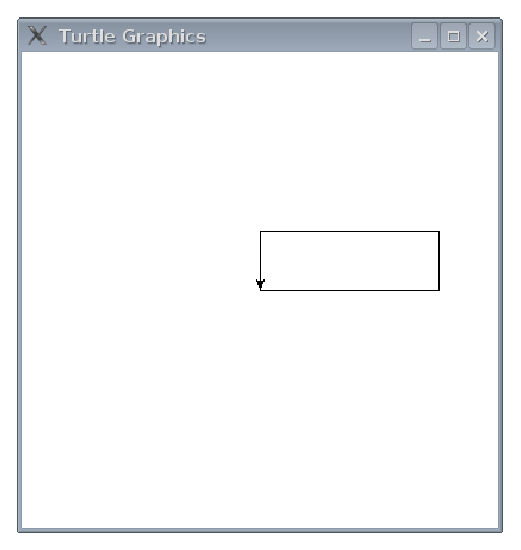
\includegraphics[width=82mm]{figure46.eps}
\end{center}
\caption{La tortuga dibujando un rectángulo.}\label{fig46}
\end{figure}

\noindent
2.   Un triángulo es un poco más complicado de dibujar, porque necesitas conocer algo más sobre ángulos y longitudes de sus lados.   Si no has estudiado aún los ángulos en el colegio, verás que es más complicado de lo que parece.   Puedes dibujar un triángulo (ver figura~\ref{fig47}) si usas el siguiente código:

\begin{listing}
\begin{verbatim}
>>> import turtle
>>> t = turtle.Pen()
>>> t.forward(100)
>>> t.left(135)
>>> t.forward(70)
>>> t.left(90)
>>> t.forward(70)
\end{verbatim}
\end{listing}

\begin{figure}
\begin{center}
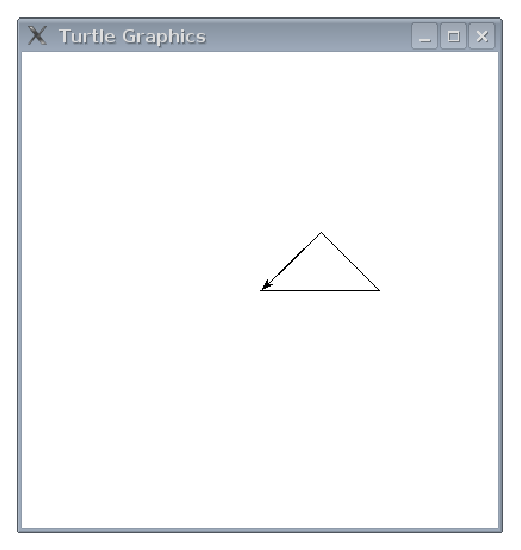
\includegraphics[width=82mm]{figure47.eps}
\end{center}
\caption{Tortuga dibujando un triángulo.}\label{fig47}
\end{figure}

\subsection*{Capítulo \ref{ch:howtoaskaquestion}}

\noindent
1.  El código del ejercicio 1 imprimirá: ``Tengo una moto''.

\noindent
El segundo ejemplo del ejercicio 1 imprimirá: ``Tengo un coche''. Ya que 80+30 no es menor que 100, lo que hace que se ejecute el código que está en el else.

\noindent
2.  Una posible respuesta para el ejercicio 2 sería:

\begin{listing}
\begin{verbatim}
>>> mivariable = 200
>>> if mivariable < 100:
...     print('hola')
... elif mivariable >= 100 and mivariable <=200:
...     print('chao')
... else:
...     print('adios')
\end{verbatim}
\end{listing}

\subsection*{Capítulo \ref{ch:againandagain}}

\noindent
1. El bucle para justo después del primer print.   Por eso cuando ejecutas el código el resultado es:

\begin{listing}
\begin{verbatim}
>>> for x in range(0, 20):
...     print('hola %s' % x)
...     if x < 9:
...         break
hola 0
\end{verbatim}
\end{listing}

\noindent
La razón por la que se para es que al principio del bucle el valor de la variable \code{x} es cero.   Como cero es un valor menor que nueve, la condición de la sentencia if es cierta, por lo que se ejecuta el código que hay dentro, el código interior es la sentencia break que sirve para decirle a Python que finalice el bucle en el que está la sentencia.

\noindent
2. Para conocer cuánto dinero consigues cuando te pagan el 3\% de interés, necesitas multiplicar el número por 0.03.   Para comenzar tendríamos que crear una variable que almacene el dinero que tenemos en nuestros ahorros.

\begin{listing}
\begin{verbatim}
>>> ahorros = 100
\end{verbatim}
\end{listing}

Para conocer el interés de un año habría que multiplicar los ahorros por 0.03:

\begin{listing}
\begin{verbatim}
>>> ahorros = 100
>>> print(ahorros * 0.03)
3.0
\end{verbatim}
\end{listing}

Son ¡3 euros!    No está mal, teniendo en cuenta que no hemos tenido que hacer nada para conseguirlo.   Necesitamos imprimir este valor y sumarlo al total de nuestros ahorros, y luego hacerlo 10 veces para saber el total que nos pagan en 10 años:

\begin{listing}
\begin{verbatim}
>>> ahorros = 100
>>> for anyo in range(1, 11):
...     interes = ahorros * 0.03
...     print('el interés ganado en el año %s es %s' % (anyo, interes))
...     ahorros = ahorros + interes
... 
el interés ganado en el año 1 es 3.0
el interés ganado en el año 2 es 3.09
el interés ganado en el año 3 es 3.1827
el interés ganado en el año 4 es 3.278181
el interés ganado en el año 5 es 3.37652643
el interés ganado en el año 6 es 3.4778222229
el interés ganado en el año 7 es 3.58215688959
el interés ganado en el año 8 es 3.68962159627
el interés ganado en el año 9 es 3.80031024416
el interés ganado en el año 10 es 3.91431955149
\end{verbatim}
\end{listing}

En la primera línea creamos un bucle for utilizando la variable \code{anyo} y la función \code{range} para contar de 1 a 10.   La segunda línea calcula el interés, multiplicando el valor de la variable \code{ahorros} por 0.03.  La siguiente línea es la sentencia print---que utiliza marcadores en la cadena de formato (\code{\%s}) para mostrar los valores del \code{anyo} e \code{interes}.  Finalmente, en la última línea, sumamos el interés a la cantidad ahorrada, lo que significa que al siguiente año el interés se calculará sobre unos ahorros mayores.
Los decimales, en el resultado, después del punto decimal, te pueden confundir un poco, pero lo que se observa es que al ir añadiendo los intereses de cada año a los ahorros, el interés que se gana cada año se va incrementando un poquito.
El código que hemos escrito podría ser un poco más útil si mostrase la cantidad ahorrada cada año:

\begin{listing}
\begin{verbatim}
>>> ahorros = 100
>>> for anyo in range(1, 11):
...     interes = ahorros * 0.03
...     print('el interés ganado para unos ahorros de %s en el año %s es %s' % 
...         (ahorros, anyo, interes))
...     ahorros = ahorros + interes
... 
el intereś ganado para unos ahorros de 100 en el año 1 es 3.0
el intereś ganado para unos ahorros de 103.0 en el año 2 es 3.09
el intereś ganado para unos ahorros de 106.09 en el año 3 es 3.1827
el intereś ganado para unos ahorros de 109.2727 en el año 4 es 3.278181
el intereś ganado para unos ahorros de 112.550881 en el año 5 es 3.37652643
el intereś ganado para unos ahorros de 115.92740743 en el año 6 es 3.4778222229
el intereś ganado para unos ahorros de 119.405229653 en el año 7 es 3.58215688959
el intereś ganado para unos ahorros de 122.987386542 en el año 8 es 3.68962159627
el intereś ganado para unos ahorros de 126.677008139 en el año 9 es 3.80031024416
el intereś ganado para unos ahorros de 130.477318383 en el año 10 es 3.91431955149
\end{verbatim}
\end{listing}

\subsection*{Capítulo \ref{ch:sortoflikerecycling}}

\noindent
1. Convertir el bucle for en una función es bastante sencillo.   La función será parecida a esto:

\begin{listing}
\begin{verbatim}
>>> def calcular_interes(ahorros, tasa):
...     for anyo in range(1, 11):
...         interes = ahorro * tasa
...         print('el interés ganado para unos ahorros de %s en el año %s es %s' % 
...             (ahorros, anyo, interes))
...         ahorro = ahorro + interes
\end{verbatim}
\end{listing}

Si comparas la función con el código anterior, te darás cuenta que, aparte de la primera línea, el único cambio al original es que en lugar de utilizar directamente el valor 0.03 como tasa de interés ahora tenemos el parámetro \code{tasa} para poder calcular para diferentes valores de tasas de interés.   Como el \code{ahorro} ya era una variable no hay que hacer ningún cambio cuando se convierte en un parámetro.   Si ejecutas esta función con los mismos valores que hemos usado hasta ahora, el resultado es el mismo que antes:

\begin{listing}
\begin{verbatim}
>>> calcular_interes(100, 0.03)
el intereś ganado para unos ahorros de 100 en el año 1 es 3.0
el intereś ganado para unos ahorros de 103.0 en el año 2 es 3.09
el intereś ganado para unos ahorros de 106.09 en el año 3 es 3.1827
el intereś ganado para unos ahorros de 109.2727 en el año 4 es 3.278181
el intereś ganado para unos ahorros de 112.550881 en el año 5 es 3.37652643
el intereś ganado para unos ahorros de 115.92740743 en el año 6 es 3.4778222229
el intereś ganado para unos ahorros de 119.405229653 en el año 7 es 3.58215688959
el intereś ganado para unos ahorros de 122.987386542 en el año 8 es 3.68962159627
el intereś ganado para unos ahorros de 126.677008139 en el año 9 es 3.80031024416
el intereś ganado para unos ahorros de 130.477318383 en el año 10 es 3.91431955149
\end{verbatim}
\end{listing}

\noindent
2. Modificar la función para pasarle el año como parámetro requiere unos cambios mínimos:

\begin{listing}
\begin{verbatim}
>>> def calcular_interes(ahorros, tasa, anyos):
...     for anyo in range(1, anyos):
...         interes = ahorro * tasa
...         print('el interés ganado para unos ahorros de %s en el año %s es %s' % 
...             (ahorros, anyo, interes))
...         ahorro = ahorro + interes
\end{verbatim}
\end{listing}

\noindent
Ahora podemos modificar la cantidad inicial, la tasa de interés y el número de años sin ningún esfuerzo:

\begin{listing}
\begin{verbatim}
>>> calcular_interes(1000, 0.05, 6)
el interés ganado para unos ahorros de 1000 en el año 1 es 50.0
el interés ganado para unos ahorros de 1050.0 en el año 2 es 52.5
el interés ganado para unos ahorros de 1102.5 en el año 3 es 55.125
el interés ganado para unos ahorros de 1157.625 en el año 4 es 57.88125
el interés ganado para unos ahorros de 1215.50625 en el año 5 es 60.7753125
\end{verbatim}
\end{listing}

\noindent
3. Este miniprograma es un poco más complicado que la función que ya hemos creado.   En primer lugar necesitamos importar el módulo sys para poder pedir por pantalla los valores con al función readline de stdin.   Aparte de esto, la función es muy similar a la anterior:

\begin{listing}
\begin{verbatim}
>>> import sys
>>> def calcular_interes():
...     print('Teclea la cantidad que tienes de ahorros:')
...     ahorros = float(sys.stdin.readline())
...     print('Teclea la tasa de interés')
...     tasa = float(sys.stdin.readline())
...     print('Teclea el número de años:')
...     anyos = int(sys.stdin.readline())
...     for anyo in range(1, anyos):
...         interes = ahorro * tasa
...         print('el interés ganado para unos ahorros de %s en el año %s es %s' % 
...             (ahorros, anyo, interes))
...         ahorro = ahorro + interes
\end{verbatim}
\end{listing}

\noindent
Cuando ejecutamos la función obtenemos algo como lo siguiente:

\begin{listingignore}
\begin{verbatim}
>>> calcular_interes()
Teclea la cantidad que tienes de ahorros:
500
Teclea la tasa de interés:
0.06
Teclea el número de años:
12
el interés ganado para unos ahorros de 500.0 en el año 1 es 30.0
el interés ganado para unos ahorros de 530.0 en el año 2 es 31.8
el interés ganado para unos ahorros de 561.8 en el año 3 es 33.708
el interés ganado para unos ahorros de 595.508 en el año 4 es 35.73048
el interés ganado para unos ahorros de 631.23848 en el año 5 es 37.8743088
el interés ganado para unos ahorros de 669.1127888 en el año 6 es 40.146767328
el interés ganado para unos ahorros de 709.259556128 en el año 7 es 42.5555733677
el interés ganado para unos ahorros de 751.815129496 en el año 8 es 45.1089077697
el interés ganado para unos ahorros de 796.924037265 en el año 9 es 47.8154422359
el interés ganado para unos ahorros de 844.739479501 en el año 10 es 50.6843687701
el interés ganado para unos ahorros de 895.423848271 en el año 11 es 53.7254308963
\end{verbatim}
\end{listingignore}

\noindent
Otra forma que tendríamos de hacer esto mismo es aprovechar la función original de cálculo de interés:

\begin{listing}
\begin{verbatim}
>>> def calcular_interes(ahorros, tasa, anyos):
...     for anyo in range(1, anyos):
...         interes = ahorro * tasa
...         print('el interés ganado para unos ahorros de %s en el año %s es %s' % 
...             (ahorros, anyo, interes))
...         ahorro = ahorro + interes
\end{verbatim}
\end{listing}

\noindent
Y crear una nueva función que se ``aproveche'' de ella. ¡Para eso son las funciones! Para reutilizar código de diversas formas. A la nueva función la vamos a llamar pedir\_y\_calcular\_interes.

\begin{listing}
\begin{verbatim}
>>> def pedir_calcular_interes():
...     print('Teclea la cantidad que tienes de ahorros:')
...     ahorros = float(sys.stdin.readline())
...     print('Teclea la tasa de interés')
...     tasa = float(sys.stdin.readline())
...     print('Teclea el número de años:')
...     anyos = int(sys.stdin.readline())
...     calcular_interes(ahorros, tasa, anyos)
\end{verbatim}
\end{listing}

\noindent
Así tenemos dos funciones, una que calcula el interés con parámetros, y otra que pide por pantalla los datos y utiliza a la primera para efectuar los cálculos.

\subsection*{Capítulo \ref{ch:turtlesgalore}}

\noindent
1. Una forma difícil de dibujar un octágono que requiere mucho que teclear:

\begin{listing}
\begin{verbatim}
import turtle
t = turtle.Pen()
>>> t.forward(50)
>>> t.right(45)
>>> t.forward(50)
>>> t.right(45)
>>> t.forward(50)
>>> t.right(45)
>>> t.forward(50)
>>> t.right(45)
>>> t.forward(50)
>>> t.right(45)
>>> t.forward(50)
>>> t.right(45)
>>> t.forward(50)
>>> t.right(45)
>>> t.forward(50)
\end{verbatim}
\end{listing}

\noindent
La tortuga se mueve 50 píxeles y luego gira 45 grados.   Lo hacemos 8 veces.   ¡Mucho que teclear!

\noindent
La forma sencila es utilizar el siguiente código:

\begin{listing}
\begin{verbatim}
>>> for x in range(0,8):
...     t.forward(50)
...     t.right(45)
\end{verbatim}
\end{listing}

\begin{figure}
\begin{center}
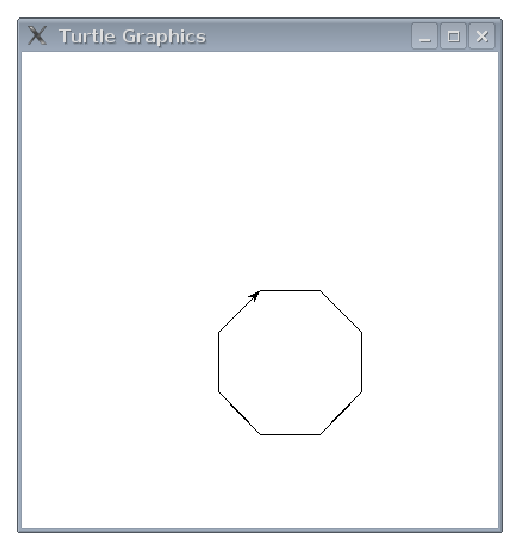
\includegraphics[width=82mm]{figure48.eps}
\end{center}
\caption{La tortuga dibujando un octágono.}\label{fig48}
\end{figure}

\noindent
2.  Si echas un vistazo a las otras funciones del Capítulo~\ref{ch:turtlesgalore}, ya sabrás como crear una forma y rellenarla.   Podemos convertir el código para crear un octágono en una función que recibe como parámetro un color.

\begin{listing}
\begin{verbatim}
>>> def octagono(red, green, blue):
...     t.color(red, green, blue)
...     t.begin_fill()
...     for x in range(0,8):
...         t.forward(50)
...         t.right(45)
...     t.end_fill()
\end{verbatim}
\end{listing}

Activamos el color, luego activamos el relleno.   Después ejecutamos el bucle para dibujar un octágono, al finalizar desactivamos el relleno.  Para probarlo vamos a dibujar un octágono azul (ver figura~\ref{fig49}):

\begin{listing}
\begin{verbatim}
>>> octagono(0, 0, 1)
\end{verbatim}
\end{listing}

\begin{figure}
\begin{center}
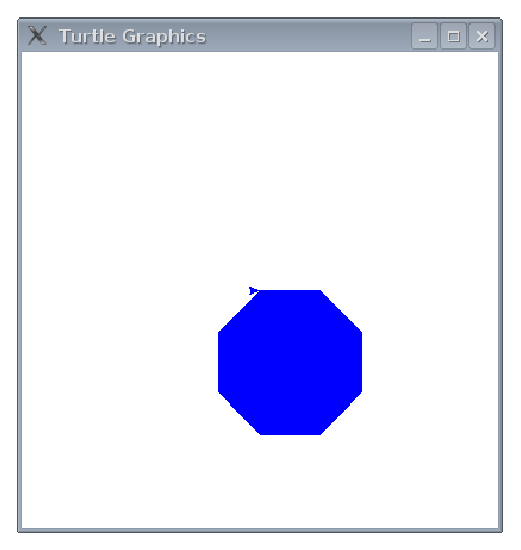
\includegraphics[width=82mm]{figure49.eps}
\end{center}
\caption{la tortuga dibujando un octágono azul.}\label{fig49}
\end{figure}
\newpage
